% Documento de tema (2--4 pp.). Mismos cinco puntos y mismo orden que slides/topic.tex.
% Todo número del modelo sale de ../code/output/topic_numbers.tex (python code/verify.py).
\documentclass[11pt]{article}
\usepackage[utf8]{inputenc}
\usepackage[T1]{fontenc}
\usepackage[spanish,es-nodecimaldot,es-noquoting]{babel}
\usepackage[margin=1in]{geometry}
\usepackage{lmodern,amsmath,amssymb,booktabs,xcolor,graphicx,colortbl}
\usepackage[colorlinks=true,allcolors=blue!50!black]{hyperref}
% Generated by python code/verify.py; do not edit numerical values by hand.
\newcommand{\PhiBase}{0.38}
\newcommand{\PhiMid}{0.50}
\newcommand{\PhiHigh}{0.70}
\newcommand{\PsiFormal}{55}
\newcommand{\PsiInformalBase}{34.00}
\newcommand{\PsiRecovered}{33.997018}
\newcommand{\PsiInformalHigh}{6.67}
\newcommand{\KappaBase}{0.4000}
\newcommand{\KappaHigh}{0.4029}
\newcommand{\TaxFormal}{0.18}
\newcommand{\NuInformal}{0.60}
\newcommand{\TimeCap}{1}
\newcommand{\MOnePercent}{51.71}
\newcommand{\MThreePP}{37.75}
\newcommand{\MThreePsiOnlyPP}{36.30}
\newcommand{\VThreeBasePP}{4.31}
\newcommand{\VThreeHighPP}{10.43}
\newcommand{\VThreeMatlabPP}{4.41}
\newcommand{\CapMassPercent}{0}
\newcommand{\MaxHoursBase}{0.75}
\newcommand{\MaxHoursHigh}{0.82}
\newcommand{\CentralProductivity}{0.8409}
\newcommand{\QOneMassPercent}{20.84}
\newcommand{\QOneMatlabMassPercent}{19.67}
\newcommand{\GridAssets}{200}
\newcommand{\GridProductivity}{40}
\newcommand{\VThreeThesisBasePP}{4.4}
\newcommand{\VThreeThesisHighPP}{10.6}
\newcommand{\QOneSharePercent}{54.3}
\newcommand{\QFiveSharePercent}{49.9}
\newcommand{\FocAPoor}{-0.2}
\newcommand{\FocARich}{12.3}
\newcommand{\FocPctFormal}{40}
\newcommand{\ShareCentralBase}{52}
\newcommand{\ShareHighPoor}{54}
\newcommand{\ShareHighRich}{47}
\newcommand{\FocPctInformalHigh}{86}
\newcommand{\IneiYear}{2017}
\newcommand{\GeAvailable}{0}
\newcommand{\GeVThreeBasePP}{4.4}
\newcommand{\GeMOneBase}{51.7}
\newcommand{\GeMThreeBase}{37.8}
\newcommand{\GeRBase}{6.60}
\newcommand{\GePIBase}{0.928}
\newcommand{\GeGiniBase}{0.521}
\newcommand{\GeSlopeBase}{0}
\newcommand{\GeVThreeMidPP}{--}
\newcommand{\GeMOneMid}{--}
\newcommand{\GeMThreeMid}{--}
\newcommand{\GeRMid}{--}
\newcommand{\GePIMid}{--}
\newcommand{\GeGiniMid}{--}
\newcommand{\GeSlopeMid}{--}
\newcommand{\GeVThreeHighPP}{--}
\newcommand{\GeMOneHigh}{--}
\newcommand{\GeMThreeHigh}{--}
\newcommand{\GeRHigh}{--}
\newcommand{\GePIHigh}{--}
\newcommand{\GeGiniHigh}{--}
\newcommand{\GeSlopeHigh}{--}
\newcommand{\GeKappaAvailable}{1}
\newcommand{\GeKappaVThreeRange}{4.37--4.39}
\newcommand{\GeVThreeBaseTwoPP}{4.41}
\newcommand{\VThreeNuOnePP}{2.3}
\newcommand{\KappaNuOne}{0.410}
\newcommand{\GiniAssets}{0.52}
\newcommand{\VThreeKappaRangeBase}{4.3--4.4}
\newcommand{\VThreeKappaRangeHigh}{10.5--10.6}
\newcommand{\KappaRangeShapes}{0.400--0.403}
\newcommand{\FrischFormalCR}{0.39}
\newcommand{\FrischInformalCR}{0.37}
\newcommand{\FrischGapCR}{$-$0.02}
\newcommand{\PhiEvidence}{0.36}
\newcommand{\VThreeEvidencePP}{4.0}
\newcommand{\KappaPercentile}{0.401}
\newcommand{\VThreePctBasePP}{4.4}
\newcommand{\VThreePctHighPP}{10.6}
\newcommand{\VSixData}{38.6}
\newcommand{\VSixModel}{6.2}
\newcommand{\VSixPercentile}{6.6}
\newcommand{\VSixAdValorem}{18.6}
\newcommand{\AdValoremMedianPercent}{94}
\newcommand{\AdValoremPsiI}{344}
\newcommand{\VThreeAdValoremPP}{13.0}
\newcommand{\VThreePercentilePP}{4.7}
\newcommand{\EduOddsData}{21}
\newcommand{\EduOddsModel}{1.6}
\newcommand{\EduRequiredRatio}{2\,926}
\newcommand{\ExtremeNodeMassPercent}{0.3}
\newcommand{\IneiQOne}{97.1}
\newcommand{\IneiQFive}{44.1}
\newcommand{\IneiQOneLatest}{94}
\newcommand{\IneiQFiveLatest}{49}
\newcommand{\IneiGapLatest}{44.7}
\newcommand{\IneiGapPreCovid}{52.6}
\newcommand{\DataMOne}{50.9}
\newcommand{\ModelMOne}{51.7}
\newcommand{\DataMTwo}{19.0}
\newcommand{\ModelMTwo}{18.8}
\newcommand{\DataMThree}{38.6}
\newcommand{\ModelMThree}{37.8}
\newcommand{\DataVOne}{2.30}
\newcommand{\ModelVOne}{2.33}
\newcommand{\DataVTwo}{1.913}
\newcommand{\ModelVTwo}{1.465}
\newcommand{\DataVThree}{53.0}
\newcommand{\ModelVThree}{4.4}
\newcommand{\DataVFour}{0.68}
\newcommand{\ModelVFour}{0.52}
\newcommand{\DataVFive}{0.40}
\newcommand{\ModelVFive}{0.22}
\newcommand{\CalibrationRows}{%
0.38 & 34.00 & 0.4000 & 4.41 \\
0.45 & 19.50 & 0.4008 & 5.77 \\
0.50 & 14.42 & 0.4013 & 6.75 \\
0.60 & 9.19 & 0.4022 & 8.68 \\
0.70 & 6.67 & 0.4029 & 10.59 \\
}

\definecolor{PaleOrange}{HTML}{FDF1E6}
\setlength{\parindent}{0pt}
\setlength{\parskip}{4pt}
\title{Ahorro, flexibilidad de horas e informalidad en el Perú\\[2pt]
\large Riqueza y reparto de horas entre el sector formal y el informal en un modelo de agentes heterogéneos}
\author{John Svante Barraza Ratachi\\
\small Track B · AI and Economic Modeling · Universidad del Pacífico\\
\small Repositorio: \url{https://github.com/johnbarraza/ai-project}}
\date{}
\begin{document}
\maketitle
\vspace{-2em}

\section{Pregunta y track}
Estudio cómo entra la riqueza en la composición de horas del hogar.
\textbf{¿Cuándo influye la riqueza en el reparto de horas entre formal e informal, para una misma productividad?}
En los datos la informalidad cae fuerte con el quintil: en 2017 la tasa de empleo informal fue \IneiQOne\,\% en el primer quintil
y \IneiQFive\,\% en el quinto (INEI, 2018, Cuadro 7.5), y en 2023, \IneiQOneLatest\,\% y \IneiQFiveLatest\,\% (figura~\ref{fig:motivation}).
El modelo de dos sectores, en cambio, genera una brecha de solo \ModelVThree{} puntos entre la fracción de horas informales del quintil
de riqueza más bajo y la del más alto. No es el mismo objeto: personas según su empleo principal frente a horas, y quintiles de gasto per cápita frente a quintiles de riqueza.

\begin{figure}[h]
\centering
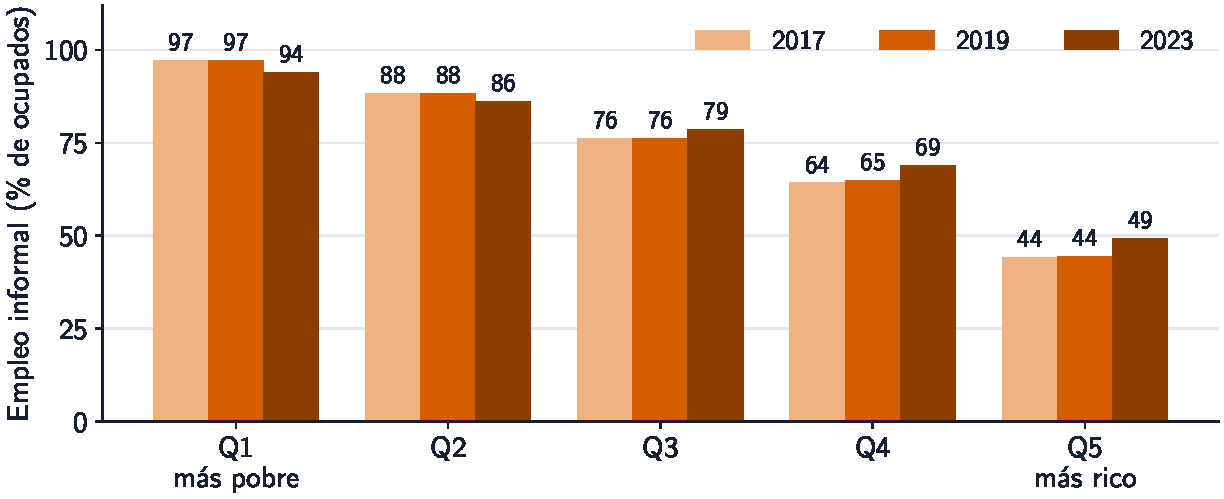
\includegraphics[width=.6\linewidth]{../code/figures/motivation_quintiles.pdf}
\caption{Tasa de empleo informal por quintil de gasto per cápita, ENAHO. Fuentes: INEI (2018, 2022); ENAHO 2023, elaboración propia.}
\label{fig:motivation}
\end{figure}

\textbf{Track B:} presento el modelo económico de \emph{Informalidad y distribución de riqueza en el Perú}.

\section{Modelo base y supuesto que cambio}
\textbf{Baseline: Aiyagari (1994).} Hogares que enfrentan shocks de productividad no asegurables ahorran por precaución;
una firma produce un bien y el ahorro agregado financia el capital ($A=K$ determina $r$). Achdou et al.\ (2022) escriben este
modelo en tiempo continuo: una ecuación de Hamilton--Jacobi--Bellman (HJB) para las decisiones y una de Kolmogorov (KF) para la distribución.
Galindo et al.\ (2024) lo aplican al Perú con formales e informales como tipos exógenos: el tipo cambia al azar y nadie lo elige.

\textbf{El supuesto que cambio: dos sectores.} Extiendo Aiyagari a dos sectores con oferta laboral endógena, dos firmas y dos bienes. El estado del hogar es $(a,z)$: los activos $a$ son endógenos
(los mueve el ahorro) y la productividad laboral individual $z$ es exógena ($\ln z$ sigue un proceso Ornstein--Uhlenbeck).
En cada instante el hogar elige consumo de bien formal $c_F$ e informal $c_I$, y horas formales $\ell_F$ e informales $\ell_I$:
\[
\max\ \mathbb E_0\!\int_0^\infty e^{-\rho t}\Big[\ln C-\sum_{s\in\{F,I\}}\frac{\psi_s\ell_s^{1+1/\phi_s}}{1+1/\phi_s}\Big]dt
\quad\text{sujeto a}
\]
\[
\dot a=R_F(z)\ell_F+R_I(z)\ell_I+ra-\chi(z)\max(-a,0)+T-c_F-p_Ic_I,
\]
con $a\ge\underline a$, $\ell_F,\ell_I\ge0$ y $\ell_F+\ell_I\le\bar H$. $C$ es una canasta CES; $\psi_s$ mide cuánto disgusta trabajar en $s$
y $\phi_s$ es la elasticidad de Frisch de esas horas. El ingreso por hora es
\[
R_F(z)=(1-\tau)w_Fz-\kappa(z),\qquad R_I(z)=\widetilde w_Iz^{\nu_I},\qquad
\kappa(z)=\kappa_{z1}\frac{z_{\max}-z}{z_{\max}-z_{\min}} .
\]
La barrera $\kappa(z)$ es una cuña por hora formal, mayor para los menos productivos. La forma lineal es la más simple decreciente
con un solo parámetro; De Soto (1986) motiva las barreras. Con forma cuadrática o raíz, recalibrada,
$\kappa_{z1}$ queda en \KappaRangeShapes{} y la brecha Q1$-$Q5 en \VThreeKappaRangeBase{} pp; con la forma por percentil $\kappa_0[1-F(z)]$,
que no depende de los extremos de la grilla, \VThreePctBasePP{} pp. Todas coinciden en $z_{\min}$ y $z_{\max}$, donde se mide M3, y como $\kappa$
depende solo de $z$, su forma no crea pendiente por riqueza.

La firma formal maximiza $A_FK_F^{\alpha}L_F^{1-\alpha}-w_FL_F-(r+\delta)K_F$, con FOC $\alpha Y_F/K_F=r+\delta$ y $(1-\alpha)Y_F/L_F=w_F$.
La informal maximiza $p_IA_IK_I^{\alpha_I}L_I^{\beta_I}-w_IL_I-(r+\delta)K_I$, con $\alpha_I p_IY_I/K_I=r+\delta$ y $\beta_Ip_IY_I/L_I=w_I$;
como $\alpha_I+\beta_I<1$, su beneficio $\Pi_I$ se reparte por hora efectiva, $\widetilde w_I=w_I+\Pi_I/L_I$. El gobierno transfiere
$T=\tau w_FL_F$. En equilibrio, $r$ iguala el ahorro de los hogares con $K_F+K_I$ y $p_I$ iguala el consumo informal con $Y_I$.

\begin{center}
\small
\renewcommand{\arraystretch}{1.12}
\begin{tabular}{@{}llrlrl@{}}
\toprule
& Momento & Dato & Fuente & Modelo & Uso\\
\midrule
M1 & Horas informales / horas totales (\%) & \DataMOne & ENAHO 2015--2019 & \ModelMOne & calibra $\psi_F,\psi_I$\\
M2 & PBI informal / PBI (\%) & \DataMTwo & INEI, Cuenta Satélite & \ModelMTwo & calibra $A_I$\\
M3 & Formalidad: $z_{\max}$ menos $z_{\min}$ (pp) & \DataMThree & EPEN 2025 & \ModelMThree & calibra $\kappa_{z1}$\\
V1 & Salario neto formal / informal & \DataVOne & BCRP & \ModelVOne & validación\\
V2 & Gasto del hogar formal / informal & \DataVTwo & ENAHO 2015--2019 & \ModelVTwo & validación\\
\rowcolor{PaleOrange} V3 & Informalidad Q1 menos Q5 (pp) & \DataVThree & INEI (2018) & \ModelVThree & no se replica\\
\rowcolor{PaleOrange} V6 & Formalidad por grupos educativos (pp) & \VSixData & EPEN 2025 & \VSixModel & no se replica\\
\bottomrule
\end{tabular}
\end{center}
M1, M3, V3 y V6 los recalcula \texttt{code/verify.py} desde la corrida exportada; M2, V1 y V2 los reporta la corrida MATLAB del modelo de dos sectores.
M3 y V6 usan el mismo dato (superior menos hasta secundaria): M3 lo compara con los nodos extremos de $z$ (\ExtremeNodeMassPercent\,\% de la masa cada uno);
V6, con grupos del peso de cada nivel en la EPEN. Con $\phi$ común, $\ell_F/\ell_I\propto(R_F/R_I)^{\phi_F}$: para que los odds de horas formales suban
\EduOddsData{} veces de primaria a universitaria, $R_F/R_I$ tendría que cambiar unas \EduRequiredRatio{} veces, lo que sugiere un margen extensivo.

\textbf{Sensibilidad: elasticidades distintas.} En el modelo de dos sectores $\phi_F=\phi_I=\PhiBase$. Aquí estudio $\phi_I>\phi_F$
para examinar cuánto depende el reparto de horas de esa igualdad. No crea tipos fijos de hogar: todos tienen los mismos $\phi_F$ y $\phi_I$,
que son propiedades de la actividad, igual que $\psi_F\neq\psi_I$ en el modelo de dos sectores; las diferencias entre hogares siguen viniendo solo de $(a,z)$.
En el modelo de dos sectores impuse $\phi_F=\phi_I$ por simplicidad; no es una normalización, porque es justamente el supuesto que cancela $V_a$.
Con la EPE de Lima, Céspedes y Rendón (2012) estiman \FrischFormalCR{} para trabajadores formales y \FrischInformalCR{} para informales
(su promedio, 0.38, es el $\phi_F$ del modelo de dos sectores). Es evidencia indirecta: compara personas distintas, no el reparto de horas de un mismo hogar
entre sectores. Por eso el rango $\phi_I\in[\PhiBase,\PhiHigh]$ es un análisis de sensibilidad (con $\phi_I=\PhiEvidence$, la brecha Q1$-$Q5 queda en \VThreeEvidencePP{} pp).

\section{Resultado esperado}
Sea $V_a=\partial v/\partial a$ el valor de un sol más de activos. Derivando la HJB respecto de $\ell_s$, con solución interior,
\begin{equation}
V_aR_s(z)=\psi_s\ell_s^{1/\phi_s}\quad\Longrightarrow\quad\ell_s=\Big(\frac{V_aR_s(z)}{\psi_s}\Big)^{\phi_s},\qquad s\in\{F,I\}:
\label{eq:foc}
\end{equation}
el beneficio marginal de una hora (su ingreso por el valor de un sol) iguala su costo marginal. Dividiendo las dos FOC,
\begin{equation}
\frac{\partial\ln(\ell_I/\ell_F)}{\partial\ln V_a}=\phi_I-\phi_F,
\qquad
\frac{\partial s_I}{\partial V_a}=s_I(1-s_I)\,\frac{\phi_I-\phi_F}{V_a},
\qquad s_I=\frac{\ell_I}{\ell_F+\ell_I}.
\label{eq:result}
\end{equation}
\textbf{Conjetura.} Si (i) la solución es interior, (ii) $R_F(z),R_I(z)>0$ y (iii) $V_a$ decrece con $a$, entonces, a igual $z$, la fracción
informal $s_I$ decrece con los activos si y solo si $\phi_I>\phi_F$. Con $\phi_I=\phi_F$, $V_a$ se cancela y la riqueza no cambia el reparto,
que es lo que ocurre en el modelo de dos sectores: su brecha V3 sale solo de que los hogares pobres tienen, en promedio, menor $z$.
\textbf{Cambio frente al modelo base:} V3 sube con $\phi_I$, manteniendo M1 y M3.

La condición (i) se cumple en la corrida del modelo de dos sectores (máximo de horas \MaxHoursBase{} con $\bar H=\TimeCap$); (iii) la verifico en la grilla
pero no la demuestro. En equilibrio parcial, con $V_a$, $g$ y precios del modelo de dos sectores y recalibrando $\psi_I$ (para M1) y $\kappa_{z1}$ (para M3),
V3 pasa de \VThreeThesisBasePP{} pp con $\phi_I=\PhiBase$ a \VThreeThesisHighPP{} pp con $\phi_I=\PhiHigh$: sube, pero queda lejos de los \DataVThree{} pp del dato.
Eso sugiere que también importa entrar o salir de la informalidad (margen extensivo), que queda fuera de este proyecto.

\section{Brecha en la literatura}
\begin{center}
\small
\renewcommand{\arraystretch}{1.12}
\begin{tabular}{@{}p{38mm}p{52mm}p{60mm}@{}}
\toprule
Trabajo & Aporte & Pendiente para mi pregunta\\
\midrule
Aiyagari (1994); Huggett (1993) & Ahorro precautorio, mercados incompletos & Un sector; sin horas formales e informales\\
Pijoan-Mas (2006) & Oferta laboral endógena: trabajar más horas también asegura & Un sector: no hay reparto\\
Meghir, Narita y Robin (2015) & Búsqueda de empleo formal e informal & Sin ahorro\\
Achdou et al.\ (2022) & El mismo modelo en tiempo continuo & Un sector\\
Galindo et al.\ (2024) & Informalidad y riqueza en el Perú, ingreso exógeno & Tipos exógenos: nadie elige ni reparte horas\\
Modelo de dos sectores & Oferta laboral endógena en dos sectores, dos firmas & $\phi$ común: la riqueza no mueve el reparto\\
\bottomrule
\end{tabular}
\end{center}
\textbf{Fuentes revisadas.} De Achdou et al.\ (2022) leí la introducción y la sección 2 (pp.~46--47 y 50--51 de la versión publicada).
De Aiyagari (1994), la ficha del working paper en el Fed de Minneapolis, no el PDF original. De Galindo et al.\ (2024), el documento (modelo, sección 2; conclusiones, sección 6) y su presentación de 2023: una economía de dotación (Huggett) con dos tipos exógenos, formal e informal, que cambian al azar y difieren en ingreso, impuesto, prima de deuda y aversión al riesgo. En sus conclusiones dejan como extensión volver endógeno el cambio entre estados, que el modelo de dos sectores hace en el margen intensivo. Del INEI (2018), el Cuadro 7.5 (p.~122 del PDF).
\textbf{Falta:} los trabajos que citan a Galindo et al.\ y evidencia de elasticidades de horas por cuenta propia frente a
asalariadas. Por eso no afirmo que el resultado sea nuevo; el registro detallado está
en \texttt{proposal/literature-check.md}.

\section{Plan y riesgos}
\textbf{Demostrar:} la ecuación (\ref{eq:result}) y la conjetura con sus tres condiciones, a mano en \texttt{hand/} y en SymPy (\texttt{code/verify.py}).
\textbf{Simular:} el equilibrio general con $\phi_I\neq\phi_F$ en el solver MATLAB del modelo de dos sectores, para ver si la pendiente sobrevive cuando $r$, $p_I$ y $V_a$
cambian. \textbf{Formalizar en Lean:} la proposición condicional, con AppliedModelingLib sobre un commit fijado de \texttt{paper/paper.pdf}.
\textbf{Estimar $\phi_I$:} en el modelo, a igual $z$, las horas solo varían por $V_a$, así que
$\mathrm{sd}(\ln\ell_I\mid z)/\mathrm{sd}(\ln\ell_F\mid z)=\phi_I/\phi_F$, medible con ENAHO dentro de cada nivel educativo.

\textbf{Paso más riesgoso:} en equilibrio general cambian $r$, $p_I$ y la distribución, y la brecha podría ser menor que en equilibrio parcial.
\textbf{Plan B:} presentar el resultado condicional y el experimento parcial como cota, declarando sus límites.

\footnotesize
\section*{Referencias}
\setlength{\parskip}{1pt}
Achdou, Y., Han, J., Lasry, J.-M., Lions, P.-L. y Moll, B. (2022). Income and wealth distribution in macroeconomics: a continuous-time approach. \emph{Review of Economic Studies}, 89(1), 45--86.\par
Aiyagari, S. R. (1994). Uninsured idiosyncratic risk and aggregate saving. \emph{Quarterly Journal of Economics}, 109(3), 659--684.\par
Céspedes, N. y Rendón, S. (2012). La elasticidad de oferta laboral de Frisch en economías con alta movilidad laboral. BCRP, Documento de Trabajo 2012-017.\par
De Soto, H. (1986). \emph{El otro sendero: la revolución informal}. Lima: El Barranco.\par
Galindo, H., Ledesma, A., Yépez, L. y Salinas, C. (2024). Informality and wealth distribution: a heterogeneous agent model. BCRP, Documento de Trabajo 2024-005.\par
Huggett, M. (1993). The risk-free rate in heterogeneous-agent incomplete-insurance economies. \emph{Journal of Economic Dynamics and Control}, 17(5--6), 953--969.\par
INEI (2018). \emph{Perú: evolución de los indicadores de empleo e ingresos por departamento, 2007--2017}. Lima: INEI.\par
INEI (2022). \emph{Perú: evolución de los indicadores de empleo e ingresos por departamento, 2007--2021}. Lima: INEI.\par
Meghir, C., Narita, R. y Robin, J.-M. (2015). Wages and informality in developing countries. \emph{American Economic Review}, 105(4), 1509--1546.\par
Pijoan-Mas, J. (2006). Precautionary savings or working longer hours? \emph{Review of Economic Dynamics}, 9(2), 326--352.\par
\textbf{Fuentes de datos.} INEI: ENAHO 2015--2019 y EPEN 2025 (microdatos de procesamiento propio), ENAHO 2021--2023 (cálculo propio); Cuenta Satélite de la Economía Informal.
Banco Mundial: World Development Indicators, índice de Gini (SI.POV.GINI), Perú 2024.\par
\end{document}
